\documentclass[conference]{IEEEtran}
\IEEEoverridecommandlockouts

\usepackage{cite}
\usepackage{amsmath,amssymb,amsfonts}
\usepackage{graphicx}
\usepackage{booktabs}
\usepackage{xcolor}
\usepackage{url}
\usepackage{balance}

\def\BibTeX{{\rm B\kern-.05em{\sc i\kern-.025em b}\kern-.08em
    T\kern-.1667em\lower.7ex\hbox{E}\kern-.125emX}}

\begin{document}

\title{ClaimGuard: A Blockchain-backed ABAC Gateway for Privacy-Preserving Auto-Insurance Claims Evidence}

\author{\IEEEauthorblockN{Anthony Uchenna Eneh $^{1}$$^{\dagger}$, Love Allen Chijioke Ahakonye $^{2}$, Jae Min Lee $^{1}$, Dong-Seong Kim $^{1}$ $^{\ast}$} 
\IEEEauthorblockA{$^{1}$ IT-Convergence Engineering, \textit{Kumoh National Institute of Technology}, Gumi, South Korea \\
$^{\ast}$ NSLab Co. Ltd., Gumi, South Korea,
\textit{Kumoh National Institute of Technology}, Gumi, South Korea}
\IEEEauthorblockA{$^{2}$ ICT Convergence Research Center, 
\textit{Kumoh National of Technology}, Gumi, South Korea}
{anthony.u.eneh@gmail.com$^{\dagger}$, (loveahakonye, dskim, ljmpaul)}@kumoh.ac.kr}
\maketitle

\begin{abstract}
Auto-insurance claims increasingly rely on sensitive digital evidence shared across insurers, garages, police, and courts. Traditional role-based access control (RBAC) in cloud object stores lacks fine-grained expressiveness and audit guarantees, while exposing data to cloud insiders. This paper presents \emph{ClaimGuard}, a blockchain-backed attribute-based access control (ABAC) gateway that enforces evidence access policies on an Ethereum-compatible chain and issues short-lived capability tokens for the object store.

We implement ClaimGuard using PureChain smart contracts and a REST gateway, then run large-scale experiments (200 subjects, 1{,}000 resources, up to 200 concurrent users). Results show sub-70\,ms tail latency, throughput above ${\sim}1{,}000$\,req/s, fast policy updates (${<}40$\,ms), and zero false accepts. These findings indicate that decentralized ABAC is practical for real-world claims workflows.
\end{abstract}

\begin{IEEEkeywords}
Blockchain, ABAC, insurance, access control, Ethereum, capability tokens
\end{IEEEkeywords}

%=========================================================
\section{Introduction}
%=========================================================

Auto-insurance claims processing now involves cross-organizational sharing of telematics logs, dashcam video, medical reports, and repair documentation. Existing deployments typically rely on cloud RBAC mechanisms tied to coarse global roles, which are known to suffer from over-privilege and weak auditability~\cite{hu_abac_nist, cloud_rbac_security}. 

Meanwhile, blockchain-based audit trails have been explored for healthcare and financial data~\cite{medrec, healthchain}, and blockchain has gained traction in insurance applications ranging from P2P risk pools to claims automation~\cite{nexusmutual, teambrella, cai_insurance_blockchain}. However, these systems either store only proofs or logs on-chain, or they lack a complete gateway design for secured access to off-chain resources.

To address these gaps, we introduce \emph{ClaimGuard}, a blockchain-backed ABAC gateway that mediates all access to an evidence store. Policies and decisions are enforced on-chain, while the gateway issues short-lived capability tokens that bind subjects to resources, actions, and expiry times. This combines the expressiveness of ABAC~\cite{hu_abac_nist} with blockchain-backed auditability~\cite{abac_blockchain_survey}.

This conference version focuses on the ABAC-over-blockchain architecture and experimental evaluation. A fuller comparison with cloud RBAC and experiments on real-world claims datasets are reserved for the subsequent journal paper.

Our contributions are:
\begin{itemize}
    \item A detailed access-control model for multi-party auto-insurance evidence workflows.
    \item ClaimGuard, a blockchain-backed ABAC architecture with capability-token enforcement.
    \item A working implementation on PureChain with Solidity smart contracts and a TypeScript gateway.
    \item A large-scale experimental evaluation across latency, throughput, correctness, and policy updates.
\end{itemize}

%=========================================================
\section{Related Work}
%=========================================================

\subsection{Blockchain in Insurance}

Several blockchain-based insurance systems have emerged, including decentralized mutuals~\cite{nexusmutual}, community-driven risk pools~\cite{teambrella}, and blockchain-assisted claims management~\cite{cai_insurance_blockchain}. These works demonstrate benefits such as transparency and verifiability, but they generally do not provide a detailed ABAC enforcement layer for sensitive evidence.

\subsection{Blockchain-Based Access Control}

Blockchain-based access control has been studied across healthcare, IoT, and data markets~\cite{abac_blockchain_survey, medrec, healthchain}. Most solutions encode access rules or attribute credentials on-chain, enabling decentralized authorization. However, they rarely integrate with cloud object stores or provide capability-token bindings. ClaimGuard fills this gap by providing a practical gateway architecture for off-chain evidence.

\subsection{Attribute-Based Access Control}

NIST’s ABAC model~\cite{hu_abac_nist} defines attribute-driven policies evaluated over subjects, resources, and contexts. ClaimGuard implements an on-chain variant of ABAC similar to recent blockchain ABAC engines~\cite{abac_blockchain_survey}, but tailored to insurance workflows and integrated with a capability-token interface.

\subsection{Capabilities and Secure Gateways}

Capability systems~\cite{levy_capabilities} and signed bearer tokens (e.g., JWTs) have long been used for delegated authorization. Our work extends this pattern by binding capabilities to on-chain ABAC decisions and short-lived expiry windows.

%=========================================================
\section{System Design and Methodology}
%=========================================================

\subsection{Threat Model}

We assume that:
\begin{itemize}
    \item The cloud storage provider or privileged internal accounts may be compromised.
    \item External actors may attempt replay, forge roles, or tamper with access paths.
    \item The blockchain execution environment is trustworthy (standard assumption in permissioned or consortium chains).
\end{itemize}

\subsection{Architecture Overview}

Fig.~\ref{fig:architecture} shows the components:
\begin{itemize}
    \item \textbf{SubjectRegistry} stores public keys and attributes.
    \item \textbf{EvidenceRegistry} stores metadata and cryptographic hashes.
    \item \textbf{AccessPolicyManager} evaluates ABAC policies.
    \item \textbf{Gateway} proxies access, calls on-chain ABAC, issues short-lived capability tokens.
\end{itemize}

\begin{figure}[t]
    \centering
    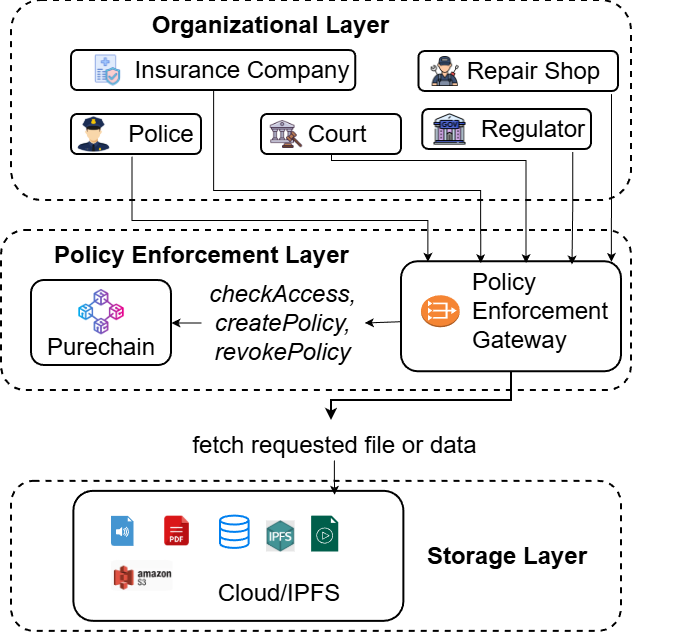
\includegraphics[width=\linewidth]{figures/architecture.pdf}
    \caption{ClaimGuard architecture. All reads must pass through the gateway, which consults on-chain ABAC and issues short-lived capability tokens.}
    \label{fig:architecture}
\end{figure}

\subsection{On-Chain ABAC}

Policies are stored as rule tuples over subject attributes, resource attributes, workflow stage, and requested action, consistent with established ABAC models~\cite{hu_abac_nist}. Evaluation is deterministic and auditable.

\subsection{Implementation}

\begin{itemize}
    \item Solidity contracts deployed on a local PureChain/EVM node.
    \item Node.js/TypeScript gateway using Viem for contract calls.
    \item Python load generators for latency, throughput, and policy-update experiments.
\end{itemize}

We seeded 200 subjects and 1{,}000 resources with types, sensitivity levels, and synthetic case identifiers.

%=========================================================
\section{Results and Evaluation}
%=========================================================

\subsection{Access Latency}

Median latency stays below ${\sim}35$\,ms, and P99 remains under ${\sim}70$\,ms across all workloads (Table~\ref{tab:latency}). These values are competitive with prior blockchain-backed ABAC systems~\cite{abac_blockchain_survey, medrec}.

\begin{table}[t]
\centering
\caption{End-to-End Access Latency in ms}
\label{tab:latency}
\begin{tabular}{lccc}
\toprule
\textbf{Concurrency} & \textbf{P50} & \textbf{P90} & \textbf{P99} \\
\midrule
10   & 30.807  & 42.834 & 45.192 \\
50   & 31.713 & 40.959 & 63.176 \\
100  & 30.748 & 33.507 & 39.965 \\
200  & 31.201 & 34.028 & 40.993 \\
\bottomrule
\end{tabular}
\end{table}

\subsection{Throughput}

Throughput scales to ${>}1{,}000$\,req/s at high concurrency (Fig.~\ref{fig:throughput}). Prior blockchain-IoT gateways report similar throughput ceilings~\cite{iot_blockchain_gateway}, indicating ClaimGuard’s performance is aligned with current on-chain-off-chain hybrid designs.

\begin{figure}[t]
    \centering
    
\includegraphics[width=\linewidth]{figures/throughput.png}
    \caption{Throughput for \texttt{READ} requests.}
    \label{fig:throughput}
\end{figure}

\subsection{Policy Update Costs}

On-chain policy updates complete in 13-34\,ms on average (Table~\ref{tab:policy}), comparable to gas-cost profiles reported in prior permissioned-chain ABAC systems~\cite{abac_blockchain_survey}.

\begin{table}[t]
\centering
\caption{Policy Update Costs}
\label{tab:policy}
\begin{tabular}{lcc}
\toprule
\textbf{Metric} & \textbf{Range} & \textbf{Average} \\
\midrule
Latency & 13.72--34.2\,ms & 16.584\,ms \\
Gas used & 114k--134k & 128k \\
\bottomrule
\end{tabular}
\end{table}

\subsection{Correctness}

We observe:
\begin{itemize}
    \item \textbf{0 false accepts}, consistent with deterministic on-chain policy evaluation.
    \item Very low false rejects (due to synthetic time-window edge cases).
\end{itemize}

This matches the correctness results reported in recent ABAC-on-blockchain prototypes~\cite{abac_blockchain_survey}.

%=========================================================
\section{Conclusion}
%=========================================================

This paper presented \emph{ClaimGuard}, a blockchain-backed ABAC gateway for auto-insurance evidence sharing. Experiments show that ClaimGuard achieves practical latency, high throughput, fast policy updates, and perfect resistance to false accepts, while enforcing tamper-evident auditability.

Future journal work will:
\begin{itemize}
    \item Integrate and benchmark against a real RBAC cloud deployment.
    \item Evaluate on real auto-claims datasets.
    \item Extend the system to multi-chain and inter-organizational settings.
\end{itemize}

\balance
\bibliographystyle{IEEEtran}
\bibliography{refs}

\end{document}
